%%% LaTeX Template: Two column article
%%%
%%% Source: http://www.howtotex.com/
%%% Feel free to distribute this template, but please keep to referal to http://www.howtotex.com/ here.
%%% Date: February 2011

%%% Preamble
\documentclass[	DIV=calc,%
							paper=a4,%
							fontsize=12pt,%
							onecolumn]{scrartcl}	 					% KOMA-article class

\usepackage{lipsum}													% Package to create dummy text
\usepackage[brazil]{babel}										% English language/hyphenation
\usepackage[protrusion=true,expansion=true]{microtype}				% Better typography
\usepackage{amsmath,amsfonts,amsthm}					% Math packages
\usepackage[pdftex]{graphicx}									% Enable pdflatex
\usepackage[svgnames]{xcolor}									% Enabling colors by their 'svgnames'
\usepackage[hang, small,labelfont=bf,up,textfont=it,up]{caption}	% Custom captions under/above floats
\usepackage{epstopdf}												% Converts .eps to .pdf
\usepackage{subfig}													% Subfigures
\usepackage{booktabs}												% Nicer tables
\usepackage{fix-cm}													% Custom fontsizes
\usepackage[utf8]{inputenc}
\usepackage[top=2.5cm, bottom=2.5cm, left=2.5cm, right=2.5cm]{geometry}
\usepackage[ddmmyyyy]{datetime}
\addto\captionsenglish{%
	\renewcommand\tablename{Tabela}
	\renewcommand\figurename{Figura}
} 
 

 
%%% Custom sectioning (sectsty package)
\usepackage{sectsty}													% Custom sectioning (see below)
\allsectionsfont{%															% Change font of al section commands
	\usefont{OT1}{phv}{b}{n}%										% bch-b-n: CharterBT-Bold font
	}

\sectionfont{%																% Change font of \section command
	\usefont{OT1}{phv}{b}{n}%										% bch-b-n: CharterBT-Bold font
	}



%%% Headers and footers
\usepackage{fancyhdr}												% Needed to define custom headers/footers
	\pagestyle{fancy}														% Enabling the custom headers/footers
\usepackage{lastpage}	

% Header (empty)
\lhead{}
\chead{}
\rhead{}
% Footer (you may change this to your own needs)

%% ====================================
%% ====================================
%% mude o rodape  do projeto
%% ====================================
%% ====================================

\lfoot{\footnotesize \texttt{Processo Unificado Adaptado} \textbullet Gerenciamento de Configuração}


\cfoot{}
\rfoot{\footnotesize página \thepage\ de \pageref{LastPage}}	% "Page 1 of 2"
\renewcommand{\headrulewidth}{0.0pt}
\renewcommand{\footrulewidth}{0.4pt}



%%% Creating an initial of the very first character of the content
\usepackage{lettrine}
\newcommand{\initial}[1]{%
     \lettrine[lines=3,lhang=0.3,nindent=0em]{
     				\color{DarkGoldenrod}
     				{\textsf{#1}}}{}}



%%% Title, author and date metadata
\usepackage{titling}															% For custom titles

\newcommand{\HorRule}{\color{DarkGoldenrod}%			% Creating a horizontal rule
									  	\rule{\linewidth}{1pt}%
										}

\pretitle{\vspace{-30pt} \begin{flushleft} \HorRule 
				\fontsize{50}{50} \usefont{OT1}{phv}{b}{n} \color{DarkRed} \selectfont 
				}

%% ====================================
%% ====================================
%% mude o titulo  do projeto
%% ====================================
%% ====================================

\title{Modelo incremental adaptado }					% Title of your article goes here

%% ====================================



\posttitle{\par\end{flushleft}\vskip 0.5em}

\preauthor{\begin{flushleft}
					\large \lineskip 0.5em \usefont{OT1}{phv}{b}{sl} \color{DarkRed}}
\author{Erik Henrique de Oliveira, Vitor Padiar Carnevalli, João Pirolo }  	% Author name goes here


\postauthor{\footnotesize \usefont{OT1}{phv}{m}{sl} \color{Black} 
					\\Universidade Tecnológica Federal do Paraná - Campus Cornélio Procópio 								% Institution of author
					\par\end{flushleft}\HorRule}

\date{}																				% No date




%%% Begin document
\begin{document}
\maketitle
\thispagestyle{fancy} 	
\thispagestyle{empty}		% Enabling the custom headers/footers for the first page 
% The first character should be within \initial{}




%% ====================================
%% ====================================
%% mude o resumo  do projeto
%% ====================================
%% ====================================
\initial{E}\textbf{este trabalho apresenta uma adaptação dos processos incremental e unificado, onde um grupo de três Eng. de Software trabalhão no processo de desenvolvimento de um produto comercial de software. } 

%% ====================================
\begin{figure}
	\centering
	
\includegraphics{utfpr}
\end{figure}

\vspace{3cm}
\centerline{\textit{\textbf{\today}}}

\clearpage
    \renewcommand*\listfigurename{Lista de figuras}
\listoffigures

\renewcommand*\listtablename{Lista de tabelas}
\listoftables




\clearpage
\renewcommand{\contentsname}{Sumário}
\tableofcontents
\clearpage

%% ====================================
%% ====================================
%% Inicio do texto
%% ====================================
%% ====================================
\section{Introdução}

O desenvolvimento de um software é uma grande tarefa que pode ser estendida por vários meses, possivelmente até um ano ou mais. Para tornar esta tarefa mais rápida e pratica é importante, dividir o trabalho em partes menores ou iterações. Cada iteração resultará num incremento ou uma versão de software. 

 Iterações são passos do e incrementos são crescimentos do produto.

O princípio do processo incremental e iterativo é que, a equipe envolvida, possa refinar e aumentar, aos poucos, a qualidade, os requisitos até atingir o sistema final.  Isso faz toda a diferença, quando falamos em grandes sistemas, a serem automatizados.   

Como o processo teve de ser adaptado a um grupo pequeno ele sofreu algumas alterações principalmente na fase de construção e transição, a nomenclatura adotada para esse modelo de processo foi: Processo Ágil Incremental adaptado.

O processo foi desenvolvido pelos desenvolvedores:
\begin{itemize}
{\item João Pirolo - Github: https://github.com/JoaoPirolo,
\item Erik Zambeli - gitHub: https://github.com/ErikZA, 
\item Vitor Padiar - GitHub: https://github.com/vitorpadiar.}
\end{itemize} 
\section{Processo}

 O Processo Unificado surgiu como um processo para o desenvolvimento de software orientados a objetos. É um processo iterativo e adaptativo de desenvolvimento que devido a maneira organizada e consistente permite conduzir um projeto de sua concepção a sua implantação.
 
 O PU utiliza um paradigma evolucionário paro o desenvolvimento de softwares. O ciclo de vida iterativo é baseado em versões e incrementos sucessivos a fim de integrar um sistema adequado. Em cada iteração incrementa-se um pouco mais o produto, baseando-se na experiência obtida nas iterações anteriores e no feedback do usuário. Cada iteração pode ser considerada uma nova versão do software de duração fixa, sendo que cada uma destas inclui suas próprias atividades de análise de requisitos, projeto, implementação e testes.
 
  Em cada iteração é escolhido um pequeno subconjunto de requisitos, os quais são rapidamente projetados, implementados e testados pelos usuários. Isso leva a uma realimentação rápida de requisitos baseada em dados concretos de usuários, desenvolvedores e testes, o PU prega uma atitude de aceitar a mudança e a adaptação como fatores inevitáveis e essenciais. Não se deve tentar especificar completamente o sistema em uma tacada interação só, essa ideia cria um conjunto congelado de requisitos.
 
 O resultado de cada iteração é um sistema executável, porém incompleto. Ele não está pronto para ser colocado em produção e pode continuar nesta situação ainda por muitas iterações mais cada iteração produz um sistema com qualidade de produto final, e não somente um protótipo.
 
  Modelo de processo unificado figura \ref{rup1}: 
 \begin{figure}
	\centering
	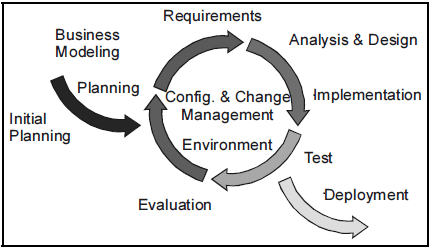
\includegraphics[]{rup1.png}
	\caption{Exemplo de Modelo Unificado}
	\label{rup1}
\end{figure}
 
 O Processo Unificado organiza suas iterações em quatro fases principais:
\begin{itemize}

\item Concepção: o objetivo desta fase é levantar, de forma genérica e pouco precisa, o escopo do projeto. Não deve existir aqui a pretensão de especificar de forma detalhada requisitos, a ideia é ter uma visão inicial do problema, estimar de forma vaga esforço e prazos e determinar se o projeto é viável e merece uma análise mais profunda.

\item Elaboração: na fase de elaboração todos (ou a grande maioria dos requisitos) são levantados em detalhes. Numa primeira iteração um ou dois requisitos, os de maior risco e valor arquitetural, são especificados em detalhes. Estes são implementados e servem como base de avaliação junto ao usuário e desenvolvedores para o planejamento da próxima iteração. Em cada nova iteração os requisitos antigos são melhor esclarecidos e novos são detalhados. Ao fim da fase, com os requisitos levantados em detalhes, os principais riscos foram tratados e pode-se então fazer estimativas mais realistas.

\item Construção: implementação iterativa dos elementos restantes de menor risco e mais fáceis e preparação para a implantação.

\item Transição: testes finais e implantação.

\end{itemize}

O Processo Unificado foi criado para ser um processo ágil de desenvolvimento e prega uma abordagem realística para a condução de um projeto. Para a sua utilização durante o desenvolvimento devido ao pequeno grupo tivemos de adaptar e modificar as atividades de suas fases para atender as necessidades do desenvolvimento.

\subsection{Papeis}

O processo original exigia a demanda de muitos papeis, para facilitar a adaptação do processo e a melhor distribuição das atividades, adotamos os seguintes papeis para nossa organização:

\begin{itemize}

	\item Gerente de Projeto: Descreve os objetivos do projeto e como ele será realizado. Inclui estimativas de custo e programação trata da identificação das atividades a serem realizadas, os artefatos e os documentos a serem produzidos, versões a serem entregues, realiza o levantamento do custo do projeto, em um segundo release acompanha o projeto de forma constante verificando o progresso e os custos  comparando com o que foi planejado inicialmente, elaboração de relatórios prestação de contas e de resultados.

	\item Analista de Sistema: levantamentos de requisitos e regras de negócio, mapeamento dos processos elaboração dos casos de uso baseado nos requisitos dos clientes, garantia da integridade dos sistemas, realizar o planejamento das versões, atua também como analista de implantação elaborando o plano de implantação da aplicação e coleta requisitos necessários para as próximas versões, aplica treinamento aos usuários.

	\item Desenvolvedor: Desenvolver, testar e liberar versões para a implantação e manter os sistemas de acordo com metodologia e técnicas propostas, para garantir a qualidade, o custo e prazo.
\end{itemize} 
\subsection{Atividades}
\begin{itemize}
    

\item Atividades do Gerente Projetos tabela \ref{tab1}:
\begin{table}[h!] % coloque h! para forcar a posicao
\centering
\caption{Modifique a legenda e crie um label}
\label{tab2} %com este label vc faz referencia no texto
\begin{tabular}{|l|l|l|l|l|}
\hline
\multicolumn{1}{|c|}{\textbf{Este é um exemplo de tabela}} & \multicolumn{2}{c|}{\textbf{C1}} & \multicolumn{2}{c|}{\textbf{C2}} \\ \hline
Você pode criar a tabela no excel                          & 1              & 2               & 3               & 4              \\ \hline
Exportar para CSV                                          & 5              & 6               & 7               & 8              \\ \hline
E importar no Table Generator                              & 9              & 10              &                 &                \\ \hline
\multicolumn{5}{|c|}{\textit{Gere o tex, e adicione em seu arquivo}}                                                             \\ \hline
\end{tabular}
\end{table}

\item Atividades do Analista de Sistemas tabela \ref{tab2}:
\begin{table}[h!]
\centering
\caption{Exemplo de tabela explicativa}
\label{tab1}
\begin{tabular}{|l|l|l|}
\hline
\multicolumn{3}{|l|}{Figura na Tabela} \\ \hline
1        & Rack          & \includegraphics[scale=0.2]{fig1}        \\ \hline
2        & Rack 2        & \includegraphics[scale=0.2]{fig1}        \\ \hline
\end{tabular}
\end{table}

\item Atividades do Desenvolvedor tabela \ref{tab3}:
\begin{table}[h!]
\centering
\caption{Tabela tarefas do Desenvolvedor}
\label{tab3}
\begin{tabular}{|l|l|l|}
\hline
\begin{tabular}[c]{@{}l@{}}Item /\\  papel\end{tabular} & Desenvolvedor                                                        & Aplicações                                                                                                                                                                                                                                                                       \\\hline
1                                                       & \begin{tabular}[c]{@{}l@{}}Desenvolver\\  o código\end{tabular}      & \begin{tabular}[c]{@{}l@{}}A atividade de desenvolver incremento de software consiste \\ em escrever o código-fonte que implementa, \\ ou corrige, um ou mais requisitos do software. \\ Esta atividade pode ser \\ realizada mais de uma vez durante uma iteração.\end{tabular} \\\hline
2                                                       & \begin{tabular}[c]{@{}l@{}}Realizar teste \\ de Unidade\end{tabular} & \begin{tabular}[c]{@{}l@{}}Trata-se de um teste do tipo estrutural \\ (caixa-branca) que deve ser produzido pelo \\ programador, em parceria com o testador, antes da \\ implementação da unidade de software.\end{tabular}                                                      \\\hline
3                                                       & \begin{tabular}[c]{@{}l@{}}Corrigir \\ Bugs\end{tabular}             & \begin{tabular}[c]{@{}l@{}}Avaliar os resultados positivos \\ e negativos dos testes.\end{tabular}                                                                                                                                                                               \\\hline
4                                                       & \begin{tabular}[c]{@{}l@{}}Integração \\ do Software\end{tabular}    & \begin{tabular}[c]{@{}l@{}}desenvolver o sistema dividindo-o em módulos ou componentes, \\  funcionalidades do componente integrado devem \\ funcionar corretamente no sistema produzido.\end{tabular}                                                                           \\\hline
5                                                       & \begin{tabular}[c]{@{}l@{}}Teste de \\ Aceitação\end{tabular}        & \begin{tabular}[c]{@{}l@{}}Nesta etapa devem ser executados os testes de sistema e, \\ se aplicáveis, os testes de aceitação.\end{tabular}                                                                                                                                       \\\hline
6                                                       & \begin{tabular}[c]{@{}l@{}}Liberação \\ da Versão\end{tabular}       & \begin{tabular}[c]{@{}l@{}}Liberar uma versão testada \\ e atualizada do Incremento\end{tabular}                                                                           \\\hline                                                                                                     
\end{tabular}
\end{table}

\end{itemize}
\section{Execução do projeto}

  Modelo do processo BPMN figura \ref{rup2}: 
 \begin{figure}
	\centering
	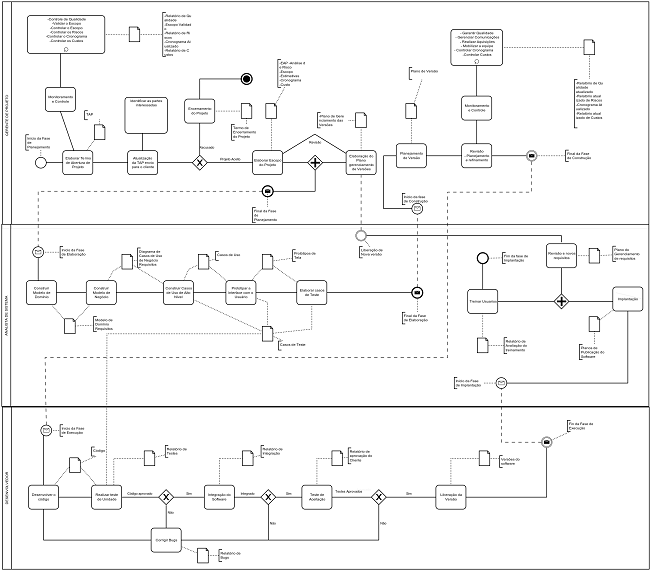
\includegraphics[]{diagram (1).png}
	\caption{Processo BPMN}
	\label{rup2}
\end{figure}

\subsection{Backlog e sprints}

    Fase de planejamento: O propósito desta fase é conseguir entendimento simultâneo entre todos os stakeholders (Gerente, Analista, Desenvolvedor) dos objetivos de ciclo de vida para o projeto, entender o que construir. Determine a Visão, o escopo do sistemas, organizações afetadas. Identifique quem é stakeholder (Cliente) do sistema assim como catalogar os riscos. Identifique as funcionalidades chave do sistema, decidir quais requisitos são mais críticos, determine pelo menos uma solução possível para os requisitos mais críticos. Identifique pelo menos uma arquitetura candidata para aplicação, entender os custos, cronograma, e os riscos associados ao projeto
Os projetos podem ter uma ou mais iterações na fase de planejamento. Entre algumas razões para ter múltiplas iterações na fase de planejamento, e que o projeto pode ser grande, e é difícil definir seu escopo. Sistema sem precedentes e muitos stakeholders (Cliente ou Organizações) com necessidades conflitantes e relacionamentos complexos. Grandes riscos técnicos que demandam a criação de um protótipo ou prova de conceito.


Fase de Elaboração: O propósito desta fase é estabelecer uma linha de base da arquitetura do sistema e prover uma base estável para o backlog de esforço de desenvolvimento na próxima fase.
O objetivo desta fase e obter um entendimento mais detalhado dos requisitos. Com um bom entendimento dos principais requisitos de negocio e domínio permite a o Analista de sistemas criar um plano mais detalhado e obter comprometimento dos stakeholders (Cliente, desenvolvedor, Gerente do projeto). Um entendimento detalhado dos requisitos é essencial pois os críticos que serão validados serão implementados primeiro no splint Backlog. O analista Projetara, implementara casos de uso, validara unidades, projetara testes e estabeleça uma linha de base para a arquitetura. Apesar da funcionalidade não estar codificada ainda, a maior parte das interfaces de usuário entre os blocos sendo construídos. Estabelecemos aqui a nossa arquitetura inicial.
O número de iterações na fase de Elaboração é dependente de fatores como desenvolvimento de um novo produto o necessidade de manutenção do sistema, sistema sem precedentes versus tecnologia e arquitetura conhecidas, podem impactar no numero de interações. 


Fase de Construção: O Gerente do projeto deve minimizar os riscos essenciais e produzir um cronograma e uma estimativa de custos precisos. Muitos riscos técnicos são resolvidos como resultado do detalhamento dos requisitos e do projeto, implementação dos casos de uso, métricas e casos de teste. Refinar e detalhe o plano de projeto. Atualizar o plano da versão de acordo com o que foi coletado na fase anterior.
A fase de Construção tem mais iterações do que as outras fases, dependendo dos tipos de projetos projeto simples, uma iteração para construir o produto (para uma liberação beta) a partir desse ponto só se faz o controle e liberação das versões. Projeto mais substancial uma iteração para expor um sistema parcial e uma para amadurecê-lo para o teste beta. Projeto grande: Três ou mais iterações, dependendo do tamanho do projeto quantidade de requisitos  elevados para uma liberação beta.


Fase de Execução: Projetar, implementar, e testar um esqueleto da estrutura do sistema de acordo com a versão proposta pelo splint backlog são tarefas do Desenvolvedor. Apesar da funcionalidade não estar completa ainda, a maior parte das interfaces entre os blocos serão construídas é implementada e testada. Isto é conhecido como uma arquitetura executável. Na primeira iteração, o desenvolvedor deve projetar, implementar, e testar um pequeno número de cenários críticos para identificar que tipo de arquitetura e mecanismos de arquitetura serão utilizados para tratar o product backlog mais critico, atuando de acordo com o plano de versões onde os backlogs com maior alto grau de complexidade serão implementados primeiro. 
Nas próximas iterações, o desenvolvedor acata os requisitos coletados pelo analista e corrige o que não estava correto na iteração anterior. O desenvolvedor projeta, implementa, e testa os cenários significantes que restaram, garantindo que todas as áreas principais do sistema foram cobertas, tratando assim os riscos potenciais o mais rápido possível para entregar a versão aos stakeholders (Clientes).


Fase de Implantação: esta fase tem como objetivo assegurar que o software esteja pronto para ser entregue aos usuários.
Implantar o sistema Beta para validar se as expectativas dos usuários foram atendidas. Isto exige ajustes finos que podem gerar novos requisitos, tais como reparação de erros e melhorias no desempenho e na usabilidade. Obter a concordância dos stakeholders (clientes) de que a distribuição está completa. Isto pode envolver vários níveis de implantação para a aceitação do produto, implantações formais, informais e testes beta. 
A fase de implantação pode incluir a execução paralela de sistemas antigos e novos, migração de dados, treinamento de usuários e ajustes nos processos de negócio. A quantidade de iterações na fase de implantação varia de uma iteração para um sistema simples que necessita primeiramente de reparos de pequenos erros, até muitas iterações para um sistema complexo, envolvendo a adição de características e a execução de atividades para fazer a transição, no negócio, do uso do sistema antigo para o sistema novo. Quando os objetivos da fase de implantação são alcançados, o projeto está pronto para ser encerrado. O fim do ciclo de vida se encerra com a implantação da versão final do software no stakeholders (clientes).

    
\subsection {Estado atual}

Artefatos gerados pelo processo em ordem cronológica tabela \ref{tab4}:
\begin{table}[h!]
\centering
\caption{Tabela Cronologia dos Artefatos}
\label{tab4}
\begin{tabular}{|l|l|l|l|}
\hline
   & Artefato                                                                  & Fase                                                                        & Papel                \\\hline
1  & TAP                                                                       & Planejamento                                                                & Gerente do Projeto   \\\hline
2  & \begin{tabular}[c]{@{}l@{}}Relatorio de qualidade\end{tabular}         & Planejamento                                                                & Gerente do Projeto   \\\hline
3  & \begin{tabular}[c]{@{}l@{}}Validação do Escopo\end{tabular}            & Planejamento                                                                & Gerente do Projeto   \\\hline
4  & \begin{tabular}[c]{@{}l@{}}Relatório de riscos\end{tabular}            & Planejamento                                                                & Gerente do Projeto   \\\hline
5  & \begin{tabular}[c]{@{}l@{}}Cronograma Atualizado\end{tabular}          & Planejamento                                                                & Gerente do Projeto   \\\hline
6  & \begin{tabular}[c]{@{}l@{}}Relatório de Custos\end{tabular}            & Planejamento                                                                & Gerente do Projeto   \\\hline
7  & EAP                                                                       & Planejamento                                                                & Gerente do Projeto   \\\hline
8  & \begin{tabular}[c]{@{}l@{}}Analise de Riscos\end{tabular}              & Planejamento                                                                & Gerente do Projeto   \\\hline
9  & Escopo                                                                    & Planejamento                                                                & Gerente do Projeto   \\\hline
10 & Estimativas                                                               & Planejamento                                                                & Gerente do Projeto   \\\hline
11 & Cronograma                                                                & Planejamento                                                                & Gerente do Projeto   \\\hline
12 & Custos                                                                    & Planejamento                                                                & Gerente do Projeto   \\\hline
13 & \begin{tabular}[c]{@{}l@{}}Gerenciamento de versões\end{tabular}       & Planejamento                                                                & Gerente do Projeto   \\\hline
14 & \begin{tabular}[c]{@{}l@{}}Requisitos de Domínio\end{tabular}          & Elaboração                                                                  & Analista de Sistemas \\\hline
15 & \begin{tabular}[c]{@{}l@{}}Requisitos de Negocio\end{tabular}          & Elaboração                                                                  & Analista de Sistemas \\\hline
16 & Casos de Uso                                                              & Elaboração                                                                  & Analista de Sistemas \\\hline
17 & \begin{tabular}[c]{@{}l@{}}Protótipos de Tela\end{tabular}             & Elaboração                                                                  & Analista de Sistemas \\\hline
18 & Casos de teste                                                            & Elaboração                                                                  & Analista de Sistemas \\\hline
19 & Plano da Versão                                                           & Construção                                                                  & Gerente do Projeto   \\\hline
20 & \begin{tabular}[c]{@{}l@{}}Relatório de qualidade\end{tabular}         & Construção                                                                  & Gerente do Projeto   \\\hline
21 & \begin{tabular}[c]{@{}l@{}}Relatório de riscos atualizado\end{tabular} & Construção                                                                  & Gerente do Projeto   \\\hline
22 & \begin{tabular}[c]{@{}l@{}}Cronograma Atualizado\end{tabular}          & Construção                                                                  & Gerente do Projeto   \\\hline
23 & \begin{tabular}[c]{@{}l@{}}Relatório de Custos atualizado\end{tabular} & Construção                                                                  & Gerente do Projeto   \\\hline
24 & Codigo                                                                    & Execução                                                                    & Desenvolvedor        \\\hline
25 & \begin{tabular}[c]{@{}l@{}}Relatório de Testes\end{tabular}            & Execução                                                                    & Desenvolvedor        \\\hline
26 & \begin{tabular}[c]{@{}l@{}}Relatório de Interações\end{tabular}        & Execução                                                                    & Desenvolvedor        \\\hline
27 & \begin{tabular}[c]{@{}l@{}}Relatório de Aprovação\end{tabular}         & Execução                                                                    & Desenvolvedor        \\\hline
28 & \begin{tabular}[c]{@{}l@{}}Relatório de Bugs\end{tabular}              & Execução                                                                    & Desenvolvedor        \\\hline
29 & \begin{tabular}[c]{@{}l@{}}Versões do Software\end{tabular}            & Execução                                                                    & Desenvolvedor        \\\hline
30 & \begin{tabular}[c]{@{}l@{}}Publicação do Software\end{tabular}         & Implantação                                                                 & Analista de Sistemas \\\hline
31 & \begin{tabular}[c]{@{}l@{}}Gerenciamento de Requisitos\end{tabular}    & Implantação                                                                 & Analista de Sistemas \\\hline
32 & Treinamentos                                                              & Implantação                                                                 & Analista de Sistemas \\\hline
\# & \begin{tabular}[c]{@{}l@{}}Liberação de \\ Versão\end{tabular}            & \begin{tabular}[c]{@{}l@{}}Retorno WorkFlow \\ de Planejamento\end{tabular} &                     \\\hline
\end{tabular}
\end{table}


\section{Referências bibliográficas}
\renewcommand\refname{} %%Referências bibliográficas}  
\bibliographystyle{ieeetr}
\begin{itemize}

\item The Unified Process Explained - Book by Kendall Scott.
\item Um Guia do Conhecimento Em Gerenciamento de Projetos - Guia Pmbok® - 5ª Ed. 2014 - Institute, Project Management.
\item Métodos Ágeis em Gerenciamento de Projetos - Rafael Dias Ribeiro,MSc,CSM,CSPO,ACP,PMP. Horácio da Cunha e Sousa Ribeiro,MSc.
\item Processo Demoiselle v1.2.3b -	https://www.frameworkdemoiselle.gov.br/

\item Desenvolvimento agil: http://www.desenvolvimentoagil.com.br/scrum

\item Noções de Engenharia de Software: http://nocoesengsw.blogspot.com/2010/03/stakeholders.html

\item Dissciplinas do Processo Unificado: http://jkolb.com.br/disciplinasfases-processo-unificado/

\end{itemize}
\bibliography{referencias}  

%% ***********************************************************************
%% === remover daqui =====================================================
%% ***********************************************************************
=================================================
\section{Elementos textuais - Tabelas}

%% ***********************************************************************
%% === ate aqui    =====  ================================================
%% ***********************************************************************

\end{document}
